\chapter{Results and Performance Evaluation}

\section{Classical Feature Engineering Results}

\subsection{Feature Correlation Matrix}

\begin{figure}[H]
\centering
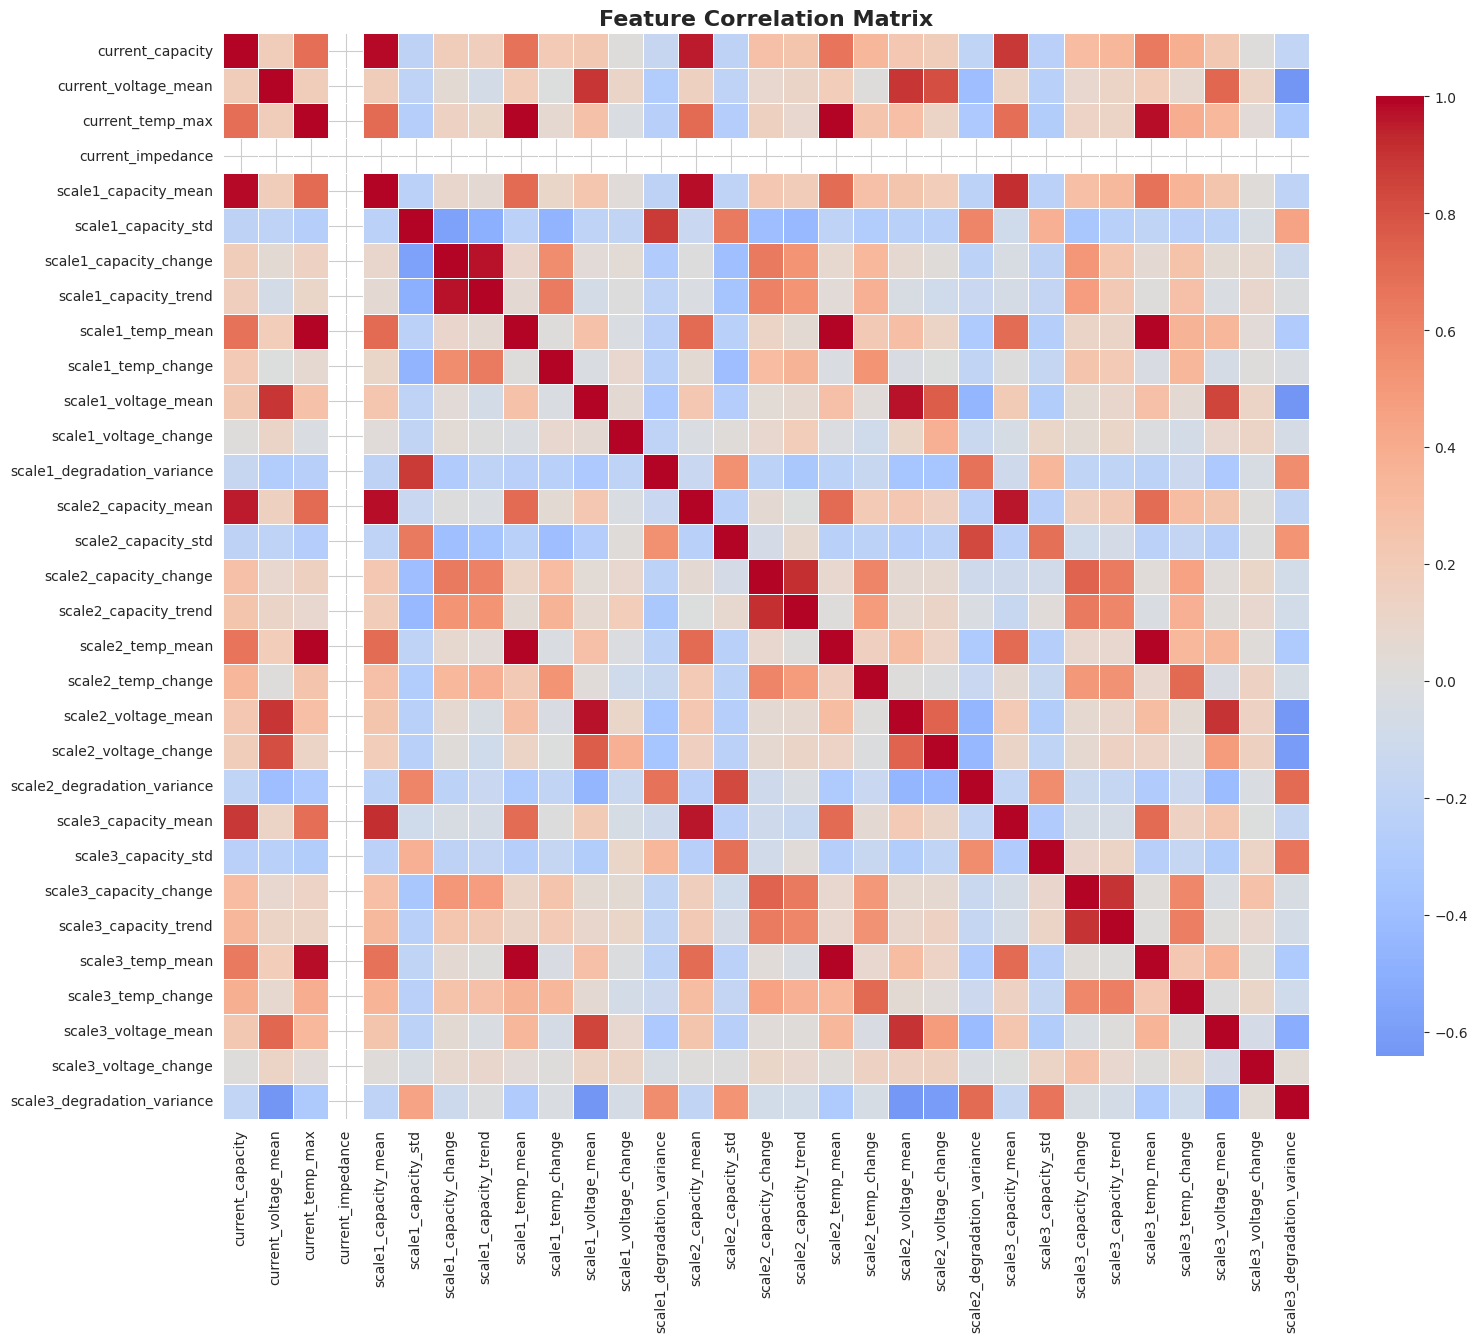
\includegraphics[width=0.75\textwidth]{Figures/8. Feature Correlation Matrix.png}
\caption{Feature Correlation Matrix}
\end{figure}

The correlation matrix illustrates relationships among statistical, impedance, and temporal degradation features.

\subsection{Key Feature Distributions}

\begin{figure}[H]
\centering
\includegraphics[width=0.75\textwidth]{Figures/8. Key Feature Distributions.png}
\caption{Key Feature Distributions}
\end{figure}

The distribution plots confirm meaningful variation in engineered features prior to quantum mapping.

\section{PCA and Quantum Feature Mapping}

\begin{figure}[H]
\centering
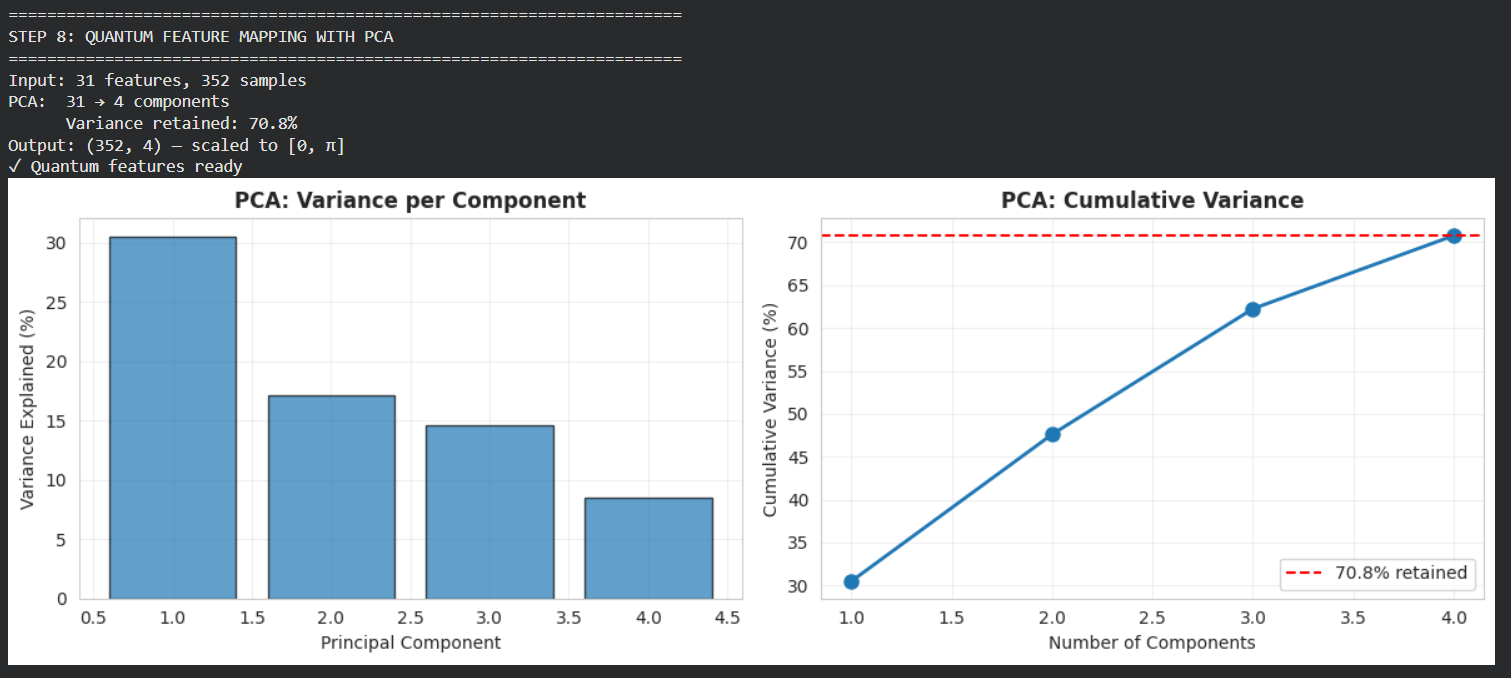
\includegraphics[width=0.7\textwidth]{Figures/9. Quantum Feature Mapping with PCA.png}
\caption{Quantum Feature Mapping with PCA}
\end{figure}

PCA reduced the classical feature space from 31 dimensions to 4 principal components for 4-qubit encoding.

\section{Quantum Kernel Construction}

\begin{figure}[H]
\centering
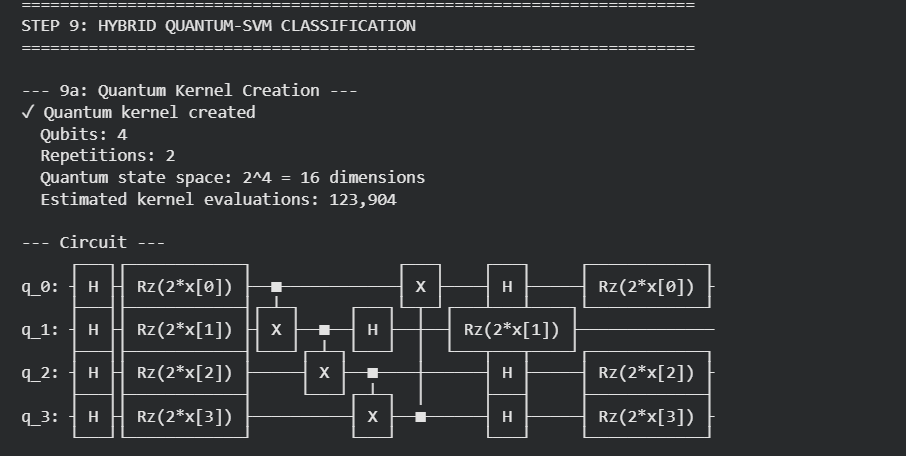
\includegraphics[width=0.7\textwidth]{Figures/10. Quantum Kernel and Circuit creation.png}
\caption{Quantum Kernel and Circuit Creation}
\end{figure}

A 4-qubit parameterized quantum circuit was constructed to encode features and compute similarity scores.

\section{Quantum Kernel Evaluation}

\begin{figure}[H]
\centering
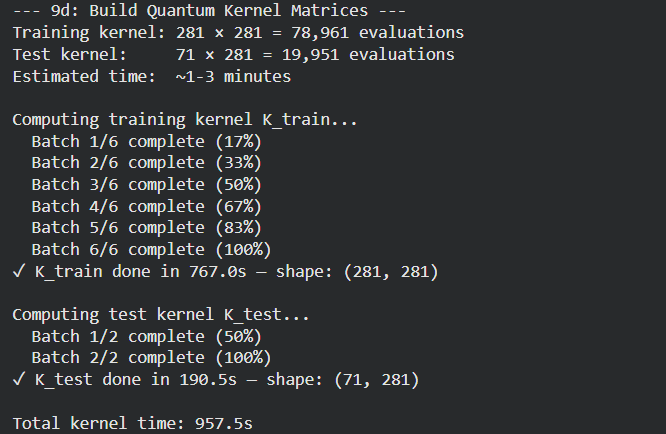
\includegraphics[width=0.7\textwidth]{Figures/12. Building Quantum kernels.png}
\caption{Building Quantum Kernel Matrix}
\end{figure}

\begin{figure}[H]
\centering
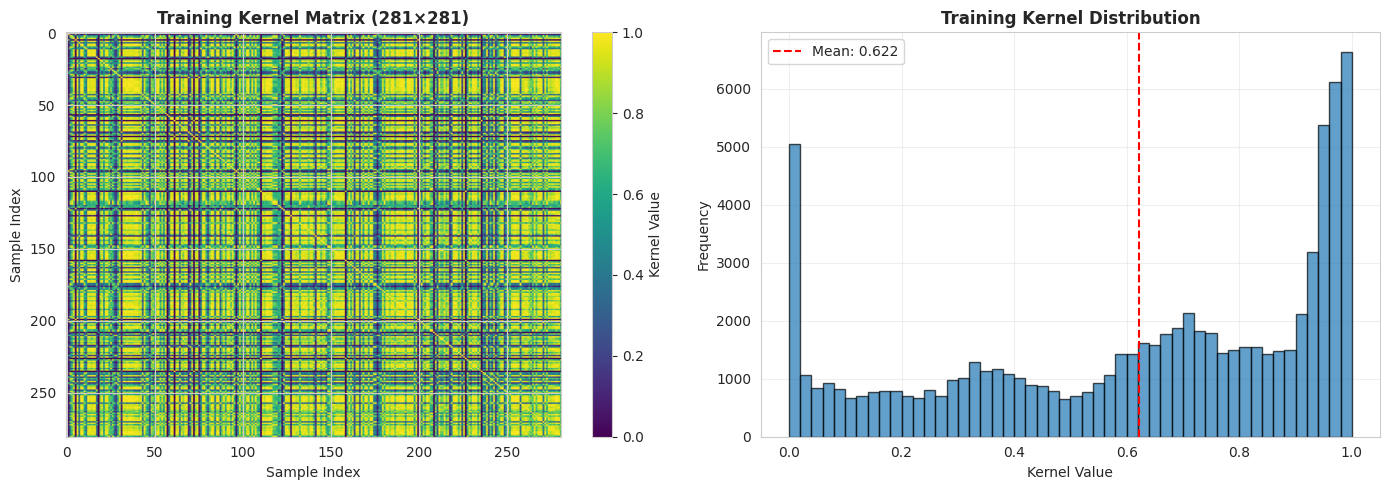
\includegraphics[width=0.7\textwidth]{Figures/12. Quantum Kernel Statistics.png}
\caption{Quantum Kernel Statistics}
\end{figure}

The kernel matrix represents similarity:

\[
K(x_i,x_j) = |\langle \psi(x_i) | \psi(x_j) \rangle|^2
\]

\section{QSVM Training and Evaluation}

\begin{figure}[H]
\centering
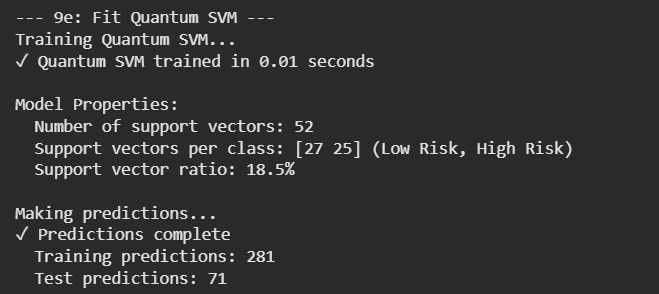
\includegraphics[width=0.7\textwidth]{Figures/13. Fit Quantum SVM.png}
\caption{Fitting Quantum SVM}
\end{figure}

\begin{figure}[H]
\centering
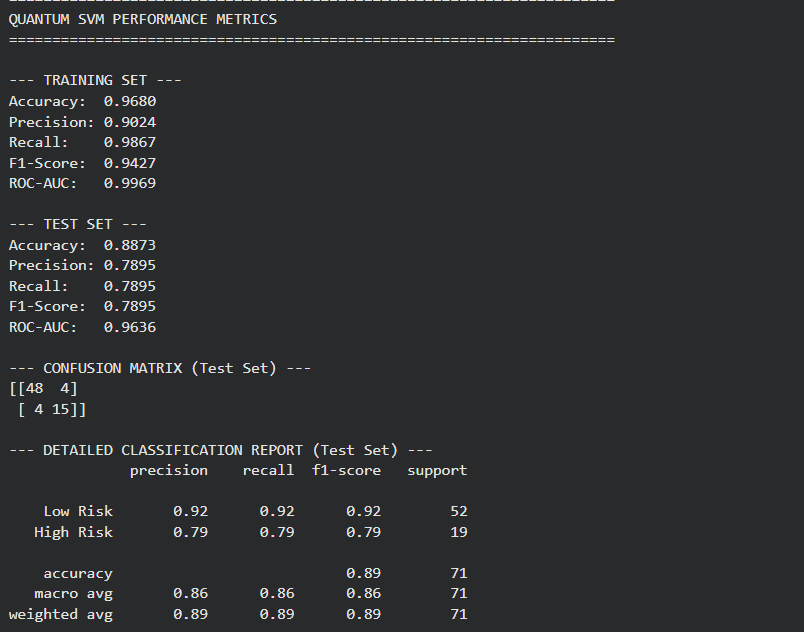
\includegraphics[width=0.7\textwidth]{Figures/14. Evaluate QSVM.png}
\caption{QSVM Evaluation}
\end{figure}

\section{Performance Metrics}

\begin{figure}[H]
\centering
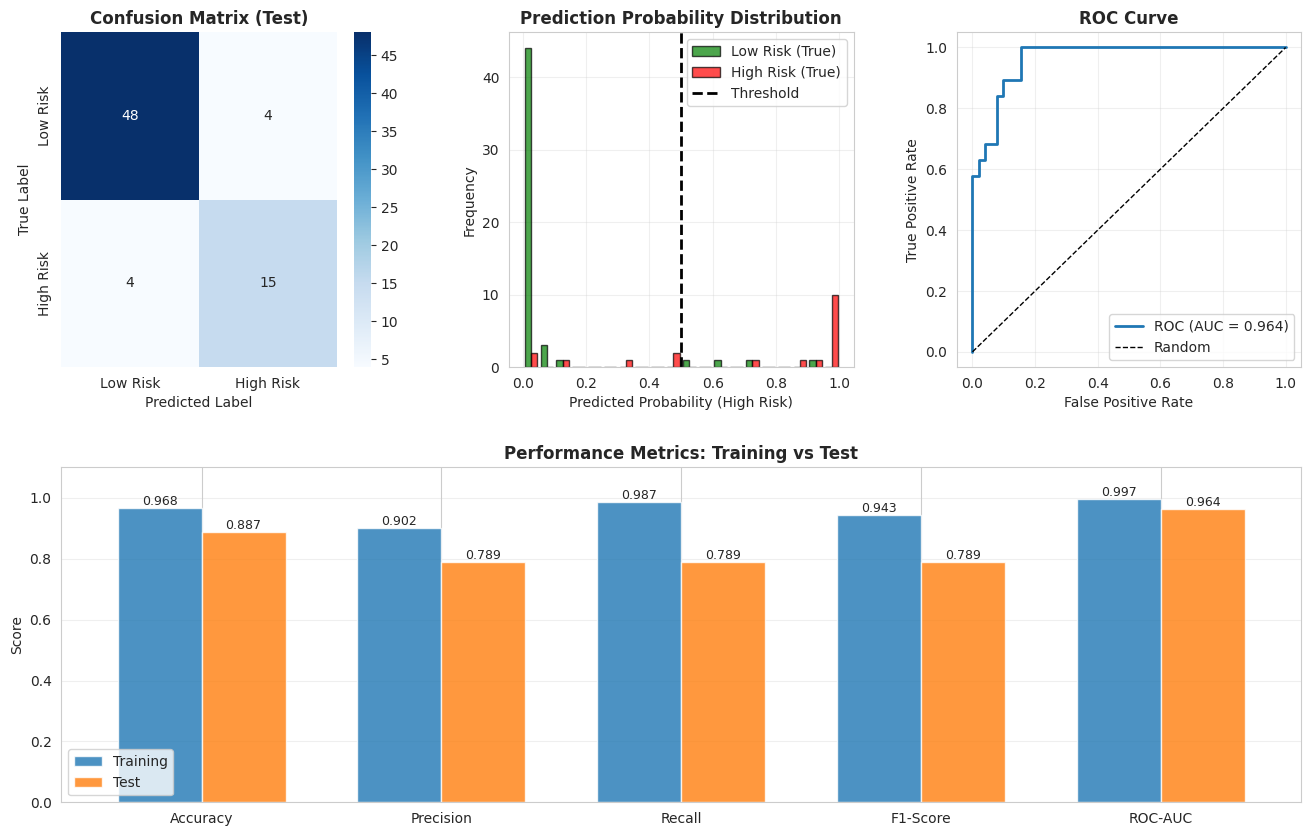
\includegraphics[width=0.7\textwidth]{Figures/15. Performance Metrics.png}
\caption{Performance Metrics of Hybrid QSVM}
\end{figure}

The model performance is evaluated using accuracy, precision, recall, and F1-score.

\section{Risk Assessment Results}

\begin{figure}[H]
\centering
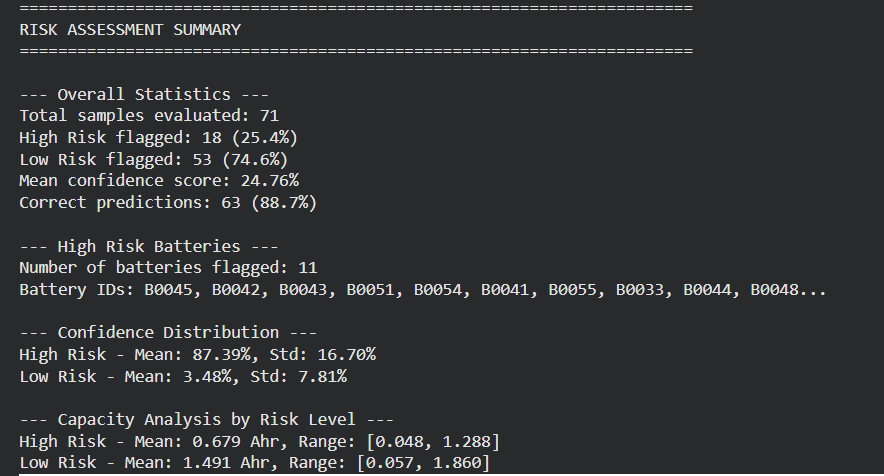
\includegraphics[width=0.7\textwidth]{Figures/16. Risk Assessment.png}
\caption{Battery Risk Assessment Output}
\end{figure}

\begin{figure}[H]
\centering
\includegraphics[width=0.7\textwidth]{Figures/16. Visualization Risk Assessment.png}
\caption{Risk Assessment Visualization}
\end{figure}

The system outputs high-risk and low-risk battery classifications along with confidence scores for monitoring applications.

\section{Summary of Results}

\begin{itemize}
\item Classical feature engineering produced meaningful degradation indicators.
\item PCA effectively reduced dimensionality for quantum encoding.
\item Quantum kernel mapping enabled nonlinear similarity modeling.
\item The hybrid QSVM achieved stable classification performance.
\item Risk outputs provide interpretable battery health monitoring.
\end{itemize}